\textbf{Data Analysis with R} is a 15 hour intensive program wherein the participants will ``learn by doing``. In this regard, two case studies will be shared, which will be prepared from 
  \begin{itemize}
    \item  \texttt{\url{https://www.kaggle.com/datasets}}
  \end{itemize}
\noindent The idea is that participants apply the techniques that they learn during the first six sessions, on the cases and prepare a presentation of their findings for the last two sessions. Also the participants will be expected to submit their R code before the last two sessions. Each case will require the participants to spend approximately 20-25 hours.

%==============================
\section*{Course Plan}
%==============================  
\begin{enumerate} 
    \item \textbf{Introduction to R (3 hours)}
     In the introduction sessions we will cover the following
    \begin{itemize}
      \item Setup R and Introduction to RStudio 
      \item Reading files in R. Introduction to data frames and basic operation on Data frames 
    \end{itemize}
    
    \item \textbf{Data Processing in R (1.5 hours)}
    
In these sessions we will cover different control structures in R. The participants will learn to write their first ``R function'' and ways to clean, aggregate and transform data:
    \item \textbf{Exploratory Data Analysis and Data Visualization in R (3 hours)}
    
In these sessions the participants will learn how to compute summary statistics of data in R, visualize datasets and learn to understand and explain ``the story of the dataset''
    \item \textbf{Statistical Modelling in R (1.5 hours)}
    
In these sessions, the participants will learn how to build a linear regression model on a multivariate dataset and interpret its results.
    \item \textbf{Case Analysis (6 hours)}
    
In these sessions, the participants will present, analyse and brainstorm on the application of different methods that they have been introduced to in the previous sessions, namely data processing, data exploration, data visualization and predictive modelling to two real world datasets.
  \end{enumerate}

%===============================  
\subsection*{The Book}
%===============================  
    % add the image of the reference book
    \begin{figure}[ht]
      \centering
      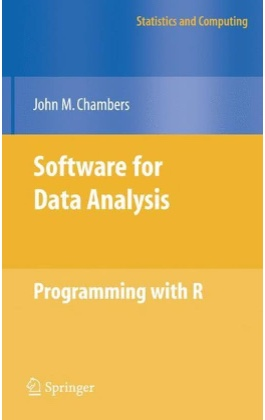
\includegraphics[width = 8 cm]{./viz/ext/book_intro_toR.jpeg}
    \end{figure}

    %add table for mapping between sessions and book 
    \begin{center}
      \begin{tabular}{ |c|c|c| } 
        \hline
          \textbf{\large Session} & \textbf{\large Chapters in the Book}  \\
        \hline   
          1 &  1, 2, 6.1, 6.2 \\
        \hline
          2 & 3, 6.3, 6.4, 6.5, 6.6, 6.7\\
        \hline  
          3 &  7 \\
        \hline
          4 & 6.8, 6.9, 6.10 \\
        \hline       
      \end{tabular}
    \end{center}
%==============================
% End of section book
%==============================

%================================
% End of chapter course overview
%=================================
